\chapter{Sonuçlar}

Geliştirmiş olduğumuz 3B-ESA-VAE modeli iyi sonuçlar üretmiştir.
Bu model Indian Pines ve Salinas veriseti üzerinde test edilmiştir. Doğruluk değerleri çeşitli
hiper parametlere göre değişmektedir. Bunun sebebi ise hızlı öğrenim yapması, aşırı öğrenme vb. olarak 
söyleyebiliriz.

\vspace{3cm}
% Side by side figures 
\begin{figure}[!ht]
    \begin{minipage}[c]{0.4\linewidth}
        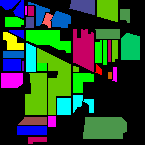
\includegraphics[width=0.7\textwidth]{Figures/IP_ground_.png}
        \caption{Indian Pines hedef sınıflandırma görüntüsü }
        \end{minipage}
    \hfill
        \begin{minipage}[c]{0.4\linewidth}
        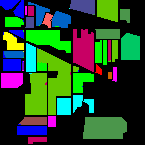
\includegraphics[width=0.7\textwidth]{Figures/IP_predicted_.png}
        \caption{Indian Pines tahmin sonucu oluşan çıktı }
    \end{minipage}%
\end{figure}

\begin{figure}[!ht]
    \begin{minipage}[c]{0.4\linewidth}
        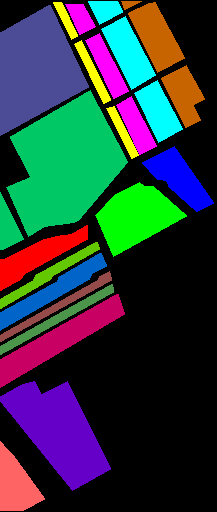
\includegraphics[width=0.7\textwidth]{Figures/SA_ground_.png}
        \caption{Salinas orjinal hedef sınıflandırma görüntüsü }
        \end{minipage}
    \hfill
        \begin{minipage}[c]{0.4\linewidth}
        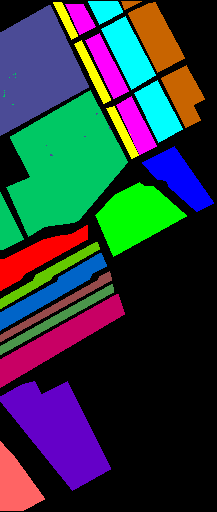
\includegraphics[width=0.7\textwidth]{Figures/SA_predicted_.png}
        \caption{Salinas tahmin sonucu oluşan çıktı }
    \end{minipage}%
\end{figure}
\newpage

\vspace{2cm}
\begin{table}[!ht]
\centering
    \begin{threeparttable} % <--- new
    \caption{Sonuçların sayısal değeleri}
        \begin{tabular}{|c|c|c|c|}
        \hline
        \textbf{Veriseti Adı} & \textbf{Kappa(\%)} & \textbf{Ortalama Doğruluk} & \textbf{Genel Doğruluk} \\ \hline
        Indian Pines & 0.989    & 99.038           & 99.038         \\ \hline
        Salinas & 0.999    & 99.881          & 99.881         \\ \hline
        \end{tabular}
    \end{threeparttable} % <--- new
\end{table}

Geliştirmiş olduğumuz modelin Tablo 5.1'de Şekil 5.2 ve Şekil 5.4 resimlerin orjinal resim ile karşılaştırmasının sayısal sonuçları verilmiştir.

